\begin{tcolorbox}
    La fonction sinus cardinal $\mathrm{sinc}:t \mapsto \frac{\sin(t)}{t}$ n'est pas intégrable sur $]0, +\infty[$.
\end{tcolorbox}

\begin{marginfigure}[-2.5cm]
    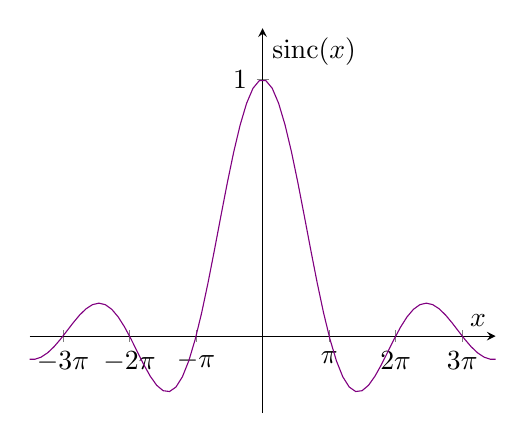
\begin{tikzpicture}
\begin{axis}[
    width=7.5cm,
    % grid=both,
    xmin=-11,
    xmax=11,
    ymin=-0.3,
    ymax=1.2,
    xlabel=$x$,
    ylabel=$\mathrm{sinc}(x)$,
    axis lines=center,
    xticklabels={$-3\pi$, $-2\pi$, $-\pi$, $\pi$, $2\pi$, $3\pi$},
    xtick={-3*3.141592, -2*3.141592, -3.141592, 3.141592, 2*3.141592, 3*3.141592},
    ytick={0, 1}
]
  \addplot[
    domain=-15:15,
    violet,
    ultra thick,
    samples=100,
  ] plot[thin] {sin(deg(x))/x};
\end{axis}
\end{tikzpicture}
\end{marginfigure}

\begin{preuve}
    On utilise le fait que pour tout $t \in \left[ \frac{\pi}{4} + k\pi, \frac{3 \pi}{4} + k \pi \right]$, $|\sin t| \geqslant \frac{1}{\sqrt{2}}$. \\
    Ainsi, pour tout $n \in \Ne$,
    \begin{align*}
        \int_{3 \pi / 4}^{n \pi + 3 \pi / 4} \left| \frac{\sin t}{t} \right| \d t &= \sum_{k=1}^n \int_{k \pi - \pi/4}^{k \pi + 3 \pi/4} \left| \frac{\sin t}{t} \right| \d t \\
        &\geqslant \frac{1}{\sqrt{2}} \sum_{k=1}^{n} \int_{k \pi - \pi/4}^{k \pi + 3 \pi/4} \frac{1}{t} \d t \\
        &\geqslant \frac{1}{\sqrt{2}} \sum_{k=1}^n \frac{\pi}{k \pi + 3 \pi/4} \\
    \end{align*}
    Or la série harmonique diverge et donc par théorème de comparaison, on obtient la non intégrabilité du sinus cardinal sur $\Rpe$.
\end{preuve}

\begin{preuve}
    Une démonstration qui ma paraît plus naturelle (\url{https://www.agreg-maths.fr/uploads/versions/1175/dirichlet.pdf}) \\
    Soit $N \in \Ne$, alors:
    \begin{align*}
        \int_0^{N \pi} \frac{|\sin x|}{x} \d x &= \sum_{k=0}^{N-1} \int_{k \pi}^{(k+1) \pi} \frac{|\sin x|}{x} \d x \\
        \text{ par changement de variable} &= \sum_{k=0}^{N-1} \int_0^\pi \frac{|\sin x|}{x + k \pi} \d x \\
        &\geqslant \sum_{k=0}^{N-1} \frac{1}{(k+1) \pi} \int_0^\pi \sin x \d x \\
        &\geqslant \frac{2}{\pi} \sum_{k=1}^N \frac{1}{k} \xrightarrow[N \to + \infty]{} + \infty.
    \end{align*}
\end{preuve}